% Options for packages loaded elsewhere
\PassOptionsToPackage{unicode}{hyperref}
\PassOptionsToPackage{hyphens}{url}
%
\documentclass[
  10pt,
]{article}
\usepackage{amsmath,amssymb}
\usepackage{iftex}
\ifPDFTeX
  \usepackage[T1]{fontenc}
  \usepackage[utf8]{inputenc}
  \usepackage{textcomp} % provide euro and other symbols
\else % if luatex or xetex
  \usepackage{unicode-math} % this also loads fontspec
  \defaultfontfeatures{Scale=MatchLowercase}
  \defaultfontfeatures[\rmfamily]{Ligatures=TeX,Scale=1}
\fi
\usepackage{lmodern}
\ifPDFTeX\else
  % xetex/luatex font selection
\fi
% Use upquote if available, for straight quotes in verbatim environments
\IfFileExists{upquote.sty}{\usepackage{upquote}}{}
\IfFileExists{microtype.sty}{% use microtype if available
  \usepackage[]{microtype}
  \UseMicrotypeSet[protrusion]{basicmath} % disable protrusion for tt fonts
}{}
\makeatletter
\@ifundefined{KOMAClassName}{% if non-KOMA class
  \IfFileExists{parskip.sty}{%
    \usepackage{parskip}
  }{% else
    \setlength{\parindent}{0pt}
    \setlength{\parskip}{6pt plus 2pt minus 1pt}}
}{% if KOMA class
  \KOMAoptions{parskip=half}}
\makeatother
\usepackage{xcolor}
\usepackage[margin=0.65in]{geometry}
\usepackage{color}
\usepackage{fancyvrb}
\newcommand{\VerbBar}{|}
\newcommand{\VERB}{\Verb[commandchars=\\\{\}]}
\DefineVerbatimEnvironment{Highlighting}{Verbatim}{commandchars=\\\{\}}
% Add ',fontsize=\small' for more characters per line
\newenvironment{Shaded}{}{}
\newcommand{\AlertTok}[1]{\textcolor[rgb]{1.00,0.00,0.00}{\textbf{#1}}}
\newcommand{\AnnotationTok}[1]{\textcolor[rgb]{0.38,0.63,0.69}{\textbf{\textit{#1}}}}
\newcommand{\AttributeTok}[1]{\textcolor[rgb]{0.49,0.56,0.16}{#1}}
\newcommand{\BaseNTok}[1]{\textcolor[rgb]{0.25,0.63,0.44}{#1}}
\newcommand{\BuiltInTok}[1]{\textcolor[rgb]{0.00,0.50,0.00}{#1}}
\newcommand{\CharTok}[1]{\textcolor[rgb]{0.25,0.44,0.63}{#1}}
\newcommand{\CommentTok}[1]{\textcolor[rgb]{0.38,0.63,0.69}{\textit{#1}}}
\newcommand{\CommentVarTok}[1]{\textcolor[rgb]{0.38,0.63,0.69}{\textbf{\textit{#1}}}}
\newcommand{\ConstantTok}[1]{\textcolor[rgb]{0.53,0.00,0.00}{#1}}
\newcommand{\ControlFlowTok}[1]{\textcolor[rgb]{0.00,0.44,0.13}{\textbf{#1}}}
\newcommand{\DataTypeTok}[1]{\textcolor[rgb]{0.56,0.13,0.00}{#1}}
\newcommand{\DecValTok}[1]{\textcolor[rgb]{0.25,0.63,0.44}{#1}}
\newcommand{\DocumentationTok}[1]{\textcolor[rgb]{0.73,0.13,0.13}{\textit{#1}}}
\newcommand{\ErrorTok}[1]{\textcolor[rgb]{1.00,0.00,0.00}{\textbf{#1}}}
\newcommand{\ExtensionTok}[1]{#1}
\newcommand{\FloatTok}[1]{\textcolor[rgb]{0.25,0.63,0.44}{#1}}
\newcommand{\FunctionTok}[1]{\textcolor[rgb]{0.02,0.16,0.49}{#1}}
\newcommand{\ImportTok}[1]{\textcolor[rgb]{0.00,0.50,0.00}{\textbf{#1}}}
\newcommand{\InformationTok}[1]{\textcolor[rgb]{0.38,0.63,0.69}{\textbf{\textit{#1}}}}
\newcommand{\KeywordTok}[1]{\textcolor[rgb]{0.00,0.44,0.13}{\textbf{#1}}}
\newcommand{\NormalTok}[1]{#1}
\newcommand{\OperatorTok}[1]{\textcolor[rgb]{0.40,0.40,0.40}{#1}}
\newcommand{\OtherTok}[1]{\textcolor[rgb]{0.00,0.44,0.13}{#1}}
\newcommand{\PreprocessorTok}[1]{\textcolor[rgb]{0.74,0.48,0.00}{#1}}
\newcommand{\RegionMarkerTok}[1]{#1}
\newcommand{\SpecialCharTok}[1]{\textcolor[rgb]{0.25,0.44,0.63}{#1}}
\newcommand{\SpecialStringTok}[1]{\textcolor[rgb]{0.73,0.40,0.53}{#1}}
\newcommand{\StringTok}[1]{\textcolor[rgb]{0.25,0.44,0.63}{#1}}
\newcommand{\VariableTok}[1]{\textcolor[rgb]{0.10,0.09,0.49}{#1}}
\newcommand{\VerbatimStringTok}[1]{\textcolor[rgb]{0.25,0.44,0.63}{#1}}
\newcommand{\WarningTok}[1]{\textcolor[rgb]{0.38,0.63,0.69}{\textbf{\textit{#1}}}}
\usepackage{longtable,booktabs,array}
\usepackage{calc} % for calculating minipage widths
% Correct order of tables after \paragraph or \subparagraph
\usepackage{etoolbox}
\makeatletter
\patchcmd\longtable{\par}{\if@noskipsec\mbox{}\fi\par}{}{}
\makeatother
% Allow footnotes in longtable head/foot
\IfFileExists{footnotehyper.sty}{\usepackage{footnotehyper}}{\usepackage{footnote}}
\makesavenoteenv{longtable}
\usepackage{graphicx}
\makeatletter
\def\maxwidth{\ifdim\Gin@nat@width>\linewidth\linewidth\else\Gin@nat@width\fi}
\def\maxheight{\ifdim\Gin@nat@height>\textheight\textheight\else\Gin@nat@height\fi}
\makeatother
% Scale images if necessary, so that they will not overflow the page
% margins by default, and it is still possible to overwrite the defaults
% using explicit options in \includegraphics[width, height, ...]{}
\setkeys{Gin}{width=\maxwidth,height=\maxheight,keepaspectratio}
% Set default figure placement to htbp
\makeatletter
\def\fps@figure{htbp}
\makeatother
\setlength{\emergencystretch}{3em} % prevent overfull lines
\providecommand{\tightlist}{%
  \setlength{\itemsep}{0pt}\setlength{\parskip}{0pt}}
\setcounter{secnumdepth}{-\maxdimen} % remove section numbering
\ifLuaTeX
  \usepackage{selnolig}  % disable illegal ligatures
\fi
\usepackage{bookmark}
\IfFileExists{xurl.sty}{\usepackage{xurl}}{} % add URL line breaks if available
\urlstyle{same}
\hypersetup{
  pdftitle={Surface and subgroup checks over GF(2\^{}83)},
  hidelinks,
  pdfcreator={LaTeX via pandoc}}

\title{Surface and subgroup checks over GF(2\^{}83)}
\author{}
\date{2026-10-12 --- run-20261012T0331Z}

\begin{document}
\maketitle

\section{Result and scope}\label{result-and-scope}

Both pinned Koblitz variants passed the native quartic-model and
subgroup checks. Each embeds into its own product and into the matching
factor of \(E_0\times E_1\), with the group law on the whole product.
The opposite pure product fails the necessary transfer conditions. These
are faithful representations of the original ECDLP; a faster solver was
not supplied or measured. The default targets were public known-answer
\(Q=37P\).

The field is \(\mathbf F_{2^{83}}\), with polynomial basis
\(z^{83}+z^{45}+z^2+z+1\). The two sources are
\(E_a:y^2+xy=x^3+ax^2+1\), \(a\in\{0,1\}\). This is an arithmetic
correctness run on one ordinary Linux x86-64 host, not an IC/rho
benchmark.

\begin{longtable}[]{@{}lrr@{}}
\toprule\noalign{}
Variant & Prime subgroup order \(r\) & Cofactor \(h\) \\
\midrule\noalign{}
\endhead
\bottomrule\noalign{}
\endlastfoot
\(a=0\) & 2417851639230796216685689 & 4 \\
\(a=1\) & 8569786107849059 & 1128547018 \\
\end{longtable}

Field degree 83 does not specify subgroup size. The \(a=0\) order has
bit length 82; the \(a=1\) order has bit length 53. The existing Sage
proof receipt is reused for both primes; the run additionally checks
\(a=1\) with deterministic u64 Miller--Rabin. No new Sage primality run
or second-host replay is claimed.

\begin{figure}
\centering
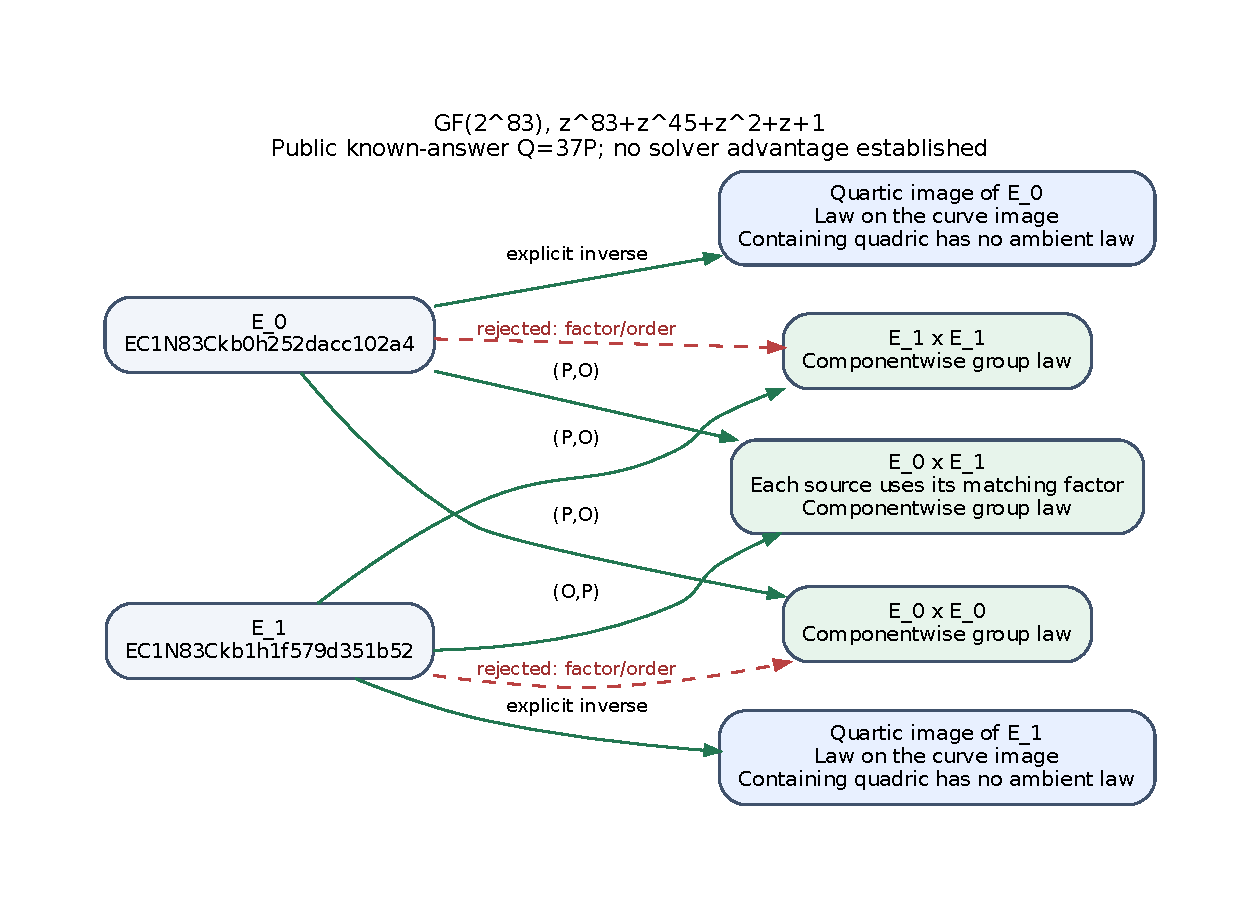
\includegraphics{destinations.pdf}
\caption{Verified inclusions and rejected opposite products. The source
labels are exact representation IDs; see the records below.}
\end{figure}

\section{What the checker actually
ran}\label{what-the-checker-actually-ran}

The modulus passed Rabin's irreducibility criterion. The Frobenius trace
recurrence reproduced the recorded orders and \(rh\). Both nonidentity
generators passed \(rP=O\); both targets passed \(rQ=O\) and the witness
check. Each source and target had Frobenius period 83. Per variant the
checker tested 166 orbit-point entries, each in its normalized and a
second projective scale, plus eight transported-addition pairs. A point
on a smooth containing quadric, outside the curve image, was rejected.

The same public targets were checked again with no scalar supplied:
subgroup membership and the transported representation passed, and
scalar-verification fields remained null. This tests the checker
interface; the target values remain known-answer fixtures, not recovered
unknown logarithms.

Four CLI controls exited with status 2: unsupported degree 82, the
two-torsion point \((0,1)\) in each odd-order subgroup, and an incorrect
scalar witness. The native package's 22 tests passed. Its controls
include independent three-word carryless multiplication and long
reduction, exhaustive curve counts over degrees 1--5, and direct
projective quadric counts over GF(2) and GF(4). The certificate
package's five tests passed, including rejection of false integer lifts
and the omitted characteristic-two correction.

\begin{figure}
\centering
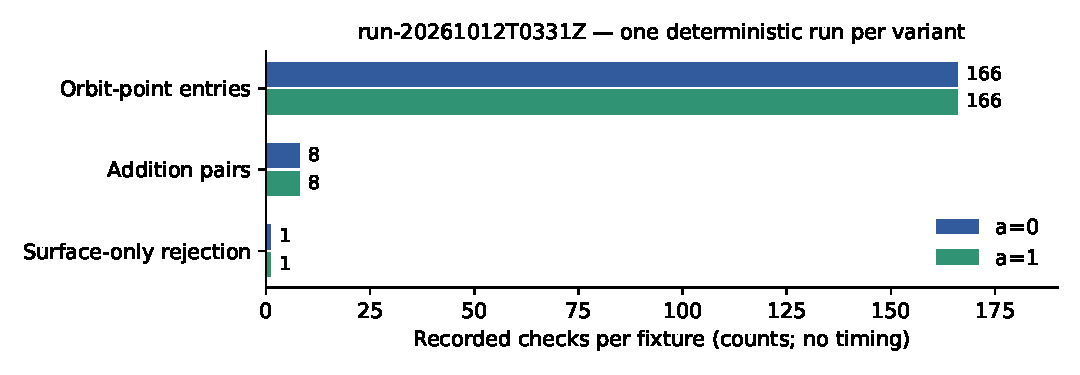
\includegraphics{checks.pdf}
\caption{Recorded verification counts, one correctness run per variant.
Entries are test populations, not distinct group states or performance
measurements.}
\end{figure}

\section{Why the characteristic-two pencil
works}\label{why-the-characteristic-two-pencil-works}

Use the embedding and its inverse

\[
(x,y)\longmapsto[1:x:y:x^2],\qquad O\longmapsto[0:0:0:1],
\]

\[
Q_1=WZ+X^2,\qquad Q_2=Y^2+XY+XZ+aWZ+W^2.
\]

Their intersection is the curve image. On \(W\ne0\), its inverse is
\((X/W,Y/W)\); on \(W=0\), the equations force \(X=Y=0\), leaving only
the origin. The transported law is
\(\operatorname{encode}(\operatorname{decode}(U)+
\operatorname{decode}(V))\). Thus the inverse preserves the source
subgroup and its ECDLP relation. A containing quadric's other points are
outside that law's domain. The control \([1:0:0:1]\) lies on the smooth
member \(\lambda=a+1\) but has \(Q_1=1\), so decoding rejects it.

For \(S_\lambda=Q_2+\lambda Q_1\), put \(c=\lambda+a\). Its polar matrix
has determinant \(c^2\). It is nonsingular for \(c\ne0\). At \(c=0\) the
point \([1:0:1:1]\) is singular. The infinite member \(Q_1\) is also
singular. Hence exactly \(q-1\) finite members are smooth, where
\(q=2^{83}\).

With \(c\ne0\), an invertible change of coordinates gives a hyperbolic
plane and the binary form

\[t^2+st+\delta_\lambda s^2,\qquad
\delta_\lambda=\lambda+c^{-2}.\]

The member is split precisely when this binary form is isotropic,
equivalently when \(u^2+u=\delta_\lambda\) has a solution. The
Artin--Schreier map has kernel \(\{0,1\}\) and image equal to the
absolute-trace-zero hyperplane. For odd degree 83 the trace map is
nonzero since \(\operatorname{Tr}(1)=1\).

For each nonzero curve coordinate \(x=c\), writing \(y=xv\) gives
\(v^2+v=x+a+x^{-2}=\delta_{a+x}\). There are two solutions exactly for a
split member. At \(x=0\) there is one point \((0,1)\), plus \(O\).
Therefore

\[\#E_a=2+2\,\#\{\text{smooth split finite members}\}.\]

The curve is defined over GF(2). With \(\tau_0=2\) and \(\tau_1=-1\) for
\(a=0\), \(\tau_1=1\) for \(a=1\), its extension traces satisfy
\(\tau_n=\tau_1\tau_{n-1}-2\tau_{n-2}\) and \(\#E_a=q+1-\tau_{83}\).
These exact counts use algebra and the recurrence; the run does not
enumerate \(2^{83}\) parameters.

\begin{longtable}[]{@{}lrr@{}}
\toprule\noalign{}
Variant & \(\#E_a\) & \(\tau_{83}\) \\
\midrule\noalign{}
\endhead
\bottomrule\noalign{}
\endlastfoot
\(a=0\) & 9671406556923184866742756 & -6151469093347 \\
\(a=1\) & 9671406556910881928556062 & 6151469093347 \\
\end{longtable}

For both variants there are \textbf{9671406556917033397649407} smooth
finite members.

\begin{longtable}[]{@{}lrr@{}}
\toprule\noalign{}
Variant & Smooth split & Smooth nonsplit \\
\midrule\noalign{}
\endhead
\bottomrule\noalign{}
\endlastfoot
\(a=0\) & 4835703278461592433371377 & 4835703278455440964278030 \\
\(a=1\) & 4835703278455440964278030 & 4835703278461592433371377 \\
\end{longtable}

\section{Product surfaces and the actual
obstruction}\label{product-surfaces-and-the-actual-obstruction}

Inclusion into \(E_a\times E_a\) is \(P\mapsto(P,O)\); projection
recovers \(P\). Inclusion into \(E_0\times E_1\) uses the matching
component. Both products have componentwise elliptic addition on every
point, and both inclusions have trivial kernel. Their Frobenius
polynomials contain the source factor by construction. They leave the
ECDLP on its original elliptic factor.

The source factors are \(\chi_i(T)=T^2-\tau_iT+q\) over the integers.
Their difference is \((\tau_1-\tau_0)T\), nonzero here, while
\(\chi_i(0)=q\ne0\). Thus they are coprime and \(\chi_a\) does not
divide \(\chi_{1-a}^2\). Also \(r_0\) does not divide \(\#E_1\) and
\(r_1\) does not divide \(\#E_0\); the recorded remainders are positive.
Since these r are prime, neither can divide the opposite order squared.
Hence the opposite product cannot receive an injective transfer of that
prime subgroup over this field.

Frobenius polynomials retain integer coefficients and trace signs; their
coefficients are not reduced modulo 2. The separate general polynomial
CLI still has u64/i128 limits. This n=83 check handles explicit
products, not arbitrary supplied large-q polynomials or new Jacobian
constructions.

\section{Identity records, representation IDs, and
replay}\label{identity-records-representation-ids-and-replay}

Six \texttt{identity.certificate/v1} records each passed exact
integer-coefficient expansion, 32 statement-derived evaluations and 32
additional evaluations. The four geometric lifts reduce modulo 2. The
normal-form integer lift carries an explicit \(2bcus\) correction, which
vanishes after reduction. The two Frobenius identities remain over the
integers. The v1 evaluator remains over \(2^{61}-1\); these records do
not claim random evaluation in GF(2\^{}83), a formal proof, or a second
host.

\begin{longtable}[]{@{}ll@{}}
\toprule\noalign{}
Identity & Certificate \\
\midrule\noalign{}
\endhead
\bottomrule\noalign{}
\endlastfoot
Quartic embedding & \texttt{IDC1h6d8ec6e3d63f147b} \\
Alternating polar determinant & \texttt{IDC1hb0891fcca2c98751} \\
Cleared-denominator normal form & \texttt{IDC1hb857d55c10efa5ac} \\
Point-count substitution & \texttt{IDC1h0869c94c259c1d1a} \\
Frobenius difference & \texttt{IDC1h4d9709f79f94a6db} \\
Frobenius product & \texttt{IDC1h240f8c156bb16781} \\
\end{longtable}

Exact record IDs are \texttt{EC1N83Ckb0h252dacc102a4} and
\texttt{EC1N83Ckb1h1f579d351b52}. Their full UID prefix is
\texttt{urn:ec-record:1:sha256:} followed by these digests:

\texttt{252dacc102a4f15413d4a269e2156852ad18dd6f8b25cf207146868c4592e2cc}

\texttt{1f579d351b52b0f3aba9259aa9b77738a958c3dbb995a6965bb50822ad199bb3}

The archived a=1 benchmark uses another polynomial basis and point
encoding. Its identifiers and targets are not substituted here. These
new exact metadata records preserve their own hash preimages; no
archived alias is reassigned.

From the repository root, reproduce the run with:

\begin{Shaded}
\begin{Highlighting}[]
\ExtensionTok{cargo}\NormalTok{ run }\AttributeTok{{-}{-}release} \AttributeTok{{-}{-}offline} \AttributeTok{{-}{-}locked} \DataTypeTok{\textbackslash{}}
  \AttributeTok{{-}{-}manifest{-}path}\NormalTok{ tools/ecdlp{-}surfaces/Cargo.toml }\DataTypeTok{\textbackslash{}}
  \AttributeTok{{-}{-}bin}\NormalTok{ binary\_surface\_check }\AttributeTok{{-}{-}} \AttributeTok{{-}{-}degree}\NormalTok{ 83 }\AttributeTok{{-}{-}a}\NormalTok{ both }\AttributeTok{{-}{-}output}\NormalTok{ /tmp/n83.json}
\ExtensionTok{cargo}\NormalTok{ run }\AttributeTok{{-}{-}release} \AttributeTok{{-}{-}offline} \AttributeTok{{-}{-}locked} \DataTypeTok{\textbackslash{}}
  \AttributeTok{{-}{-}manifest{-}path}\NormalTok{ docs/ecdlp{-}surfaces/certificates/Cargo.toml }\DataTypeTok{\textbackslash{}}
  \AttributeTok{{-}{-}bin}\NormalTok{ binary\_identities }\AttributeTok{{-}{-}}\NormalTok{ /tmp/n83.json /tmp/n83{-}identities}
\ExtensionTok{tools/ecdlp{-}surfaces/check.sh}
\end{Highlighting}
\end{Shaded}

Raw evidence: \href{../../runs/run-20261012T0331Z/n83.json}{both cases},
\href{../../runs/run-20261012T0331Z/no_witness_a0.json}{no-witness a=0},
\href{../../runs/run-20261012T0331Z/no_witness_a1.json}{no-witness a=1},
\href{../../runs/run-20261012T0331Z/identities/identity_replay.json}{identity
replay},
\href{../../runs/run-20261012T0331Z/identities/curve_record_a0.json}{a=0
curve record},
\href{../../runs/run-20261012T0331Z/identities/curve_record_a1.json}{a=1
curve record},
\href{../../runs/run-20261012T0331Z/source_and_binary.sha256}{source and
binary hashes}, and the
\href{../../runs/run-20261012T0331Z/manifest.json}{run manifest}.

The full \texttt{crypto} library gate was attempted and remains blocked
by its preexisting syntax error in the Koblitz factor-base source, line
1854
(\href{../../runs/run-20261012T0331Z/root_library_gate.log}{diagnostic}).
Its source is unchanged. Conductor is unavailable. An initial launch
used a root-relative manifest from the crate directory and failed with
exit 101; the corrected commands above passed. That failure and the
preliminary smoke output are retained separately from the final recorded
evidence.

No IC candidate, isogeny route, performance row, or subgroup-size
promotion is made. Canonical graph and registry checks are recorded in
\texttt{GRAPH\_REVIEW.md}. Arbitrary surface homomorphisms,
target-solver cost, and any ECDLP advantage remain unresolved. No task
is scheduled after this report.

\section{Sources}\label{sources}

\begin{itemize}
\tightlist
\item
  \href{https://www.secg.org/sec1-v2.pdf}{SEC 1 v2, §§2.1.2 and 2.2.2}:
  polynomial-basis binary arithmetic and the elliptic addition formulas
  used here.
\item
  \href{https://github.com/aburan28/crypto/blob/8f7f796d694fd41b4db81b25c1aff3632d012c65/src/cryptanalysis/koblitz_index_calculus.rs\#L975}{Pinned
  n=83 fixtures}: exact source generators, orders and cofactors.
\item
  \href{https://github.com/aburan28/crypto/blob/8f7f796d694fd41b4db81b25c1aff3632d012c65/research/f6_wide_n83_20261004/prime-check.txt}{Existing
  prime-proof receipt} and
  \href{https://github.com/aburan28/crypto/blob/8f7f796d694fd41b4db81b25c1aff3632d012c65/research/f6_wide_n83_20261004/prime_check.sage}{checked-Sage
  source}: reused proof evidence; local copies and hashes accompany this
  study.
\item
  \href{https://math.mit.edu/classes/18.783/2023/LectureNotes13.pdf}{Sutherland,
  MIT 18.783, Lecture 13}: Frobenius characteristic-polynomial
  framework. The extension trace recurrence and binary classification
  are derived explicitly above.
\item
  \href{../../../../tools/ecdlp-surfaces/src/binary.rs}{Native checker},
  \href{../../../../tools/ecdlp-surfaces/tests/binary.rs}{independent
  native controls}, and
  \href{../../../../docs/ecdlp-surfaces/certificates/src/bin/binary_identities.rs}{integer-lift
  checker}.
\end{itemize}

\end{document}
